\documentclass{article}

% Language setting
% Replace `english' with e.g. `spanish' to change the document language
\usepackage[english]{babel}

% Set page size and margins
% Replace `letterpaper' with`a4paper' for UK/EU standard size
\usepackage[letterpaper,top=2cm,bottom=2cm,left=3cm,right=3cm,marginparwidth=1.75cm]{geometry}

% Useful packages
\usepackage{amsmath}
\usepackage{graphicx}
\usepackage[colorlinks=true, allcolors=blue]{hyperref}

\title{A Comparitive Study Between Gaming And Gambling}
\author{Pranveer Singh}



\begin{document}
\maketitle



\begin{abstract}

This article discusses the history of gambling and research done on its effects on society, and applies its conclusions onto modern-day gaming to verify if the current state of gaming is akin to gambling, or features bordering close. This is done by interconnecting several studies and their analysis. It also aims to raise awareness towards possibly unethical practices in the gaming industry, and their outcomes, especially on children. The article concludes by attempting to provide possible resolutions towards a safer gaming experience.

\end{abstract}

\section{Introduction}
Since the start of this century, we live in a world saturated with technology. Technology is foundational to modern day society. Today, an average human cannot help but to interact with some form of technology daily, that is, it is unavoidable.
This technology is also our method of connecting to the Internet. With the advent of the internet, we are able to operate in a way that would seem nothing but magical to someone over a few decades ago. Society has undeniably evolved through this, and although there are endless positives to this advancement, this report will shine light to a possibly overlooked con of this development.\cite{walker1992psychology}

The goal of this report is to compare the recent trends in \textbf{Gaming} and adjacent concepts with the established and well researched industry of \textbf{Gambling}. A gamble is defined as "an act having an element of risk" and thus gambling is formally defined as "the practice or activity of betting : the practice of risking money or other stakes in a game or bet". Traditional gambling is well known to be risky, and yet addictive. In fact, it was a highly prominent form of "gaming" in the 19th and 20th century. \cite{parker2008problem} \cite{dowling2005electronic}

The scope of this report is far narrower than what is presumed above, yet this comparison between gaming and gambling may shine a light on the ethics of the industry and whether gaming needs restrictions similar to gambling.

\section{Gambling}
Gambling in various forms has been around throughout recorded history,
but in-depth scholarship on it is a recent phenomenon occasioned by the
resurgence of widespread gambling in America in the 1980s and 90s. The
four books reviewed here approach the topic from different scholarly angles:
the legal history of gambling in America, history of the practice and the
business of gambling, focused assessment of the risks and benefits of gambling, and the moral evaluation of gambling. Some of the authors remain
more optimistic about the practice’s contribution to society, while others
focus on potential harmful consequences of the human desire to gamble.
Together they provide insight about the complex history of gambling and
speculation about why humans play games of chance.\cite{kuss2012online} \cite{kuss2013internet} \cite{national1999pathological}

Gambling which has been primarily thought of as an adult activity
has recently been shown to be a popular activity amongst the young. As there are few observable signs of gambling dependence among children and adolescents, such problems frequently go undetected compared to other forms of addiction (e.g.
substance abuse. Nevertheless, retrospective studies indicate that adult problem gamblers report the onset of their pathological behaviors to have begun between the ages of 10-19. Family members of pathological gamblers may also be more susceptible to problems such that 20-25 percent of their children gamble themselves and/or show other forms of addictions.\cite{ko2009brain}\cite{young2009understanding} \cite{parker2008problem}

\section{Gaming and Video Gaming}
The use of video-games is very prevalent in our society. Regardless of socioeconomic status, home consoles (e.g. Xbox, Playstation or personal computers which act as video-game devices) remain popular. Like gambling, video-games are reinforcing because they sharpen the contingencies of winning and losing. Some researchers have speculated that commercial video-games make use of similar types of 'addictive' reinforcement schedules as do gambling activities and that video players manifest compulsive tendencies in their play. Compulsive or excessive video-game playing shares many properties with other addictions. Individuals report feelings of excitement when playing (similar to an adrenaline rush), it is often engaged in for the purpose of relieving stress, it has a strong learning component, and it is commonly regarded as a form of sensation seeking.\cite{dowling2005electronic} \cite{king2020convergence}

\section{Fundamental Difference between Gaming and Gambling}
Despite the similarities above, the key difference lies in the flow of money. Lets take an example of a slot machine in an actual casino, and an offline slot machine "game" bought from a store. Both function the exact same way in terms of the rules of the use. In an actual casino, each run of machine requires additional money or its substitute. Thus, the more addictive the machine is, the more revenue is generated. On the other hand,in the video game version, you get to have infinite runs, all for the single payment made at the purchase of the game (despite any alternate method to add friction per run such as a time-out or prerequisite challenge).Thus, the game designer is not monetarily motivated to make the game more addictive, and rather incentivised to make the overall experience enjoyable to sell more versions of the game.This should help draw an effective line to assess the morality of the medium of entertainment.Unfortunately, a certain innovation discussed below has blurred this line for the past few years.\cite{gainsbury2015exploratory} 

\section{Micro-transactions and Other Systems}

\subsection{Microtransactions}
Lets make a slight modification to the example above. Instead of the slot machine video game to be only a one-time purchase, it is now online and thus allows you to upgrade the game via further add-on purchases. Now you can have a better experience by paying more.Suddenly, the key difference mentioned in heading 4 dissapears. There is no functional difference between this game and an actual slot machine.

This is what is known as a Microtransaction.Since the advent of online gaming, devs found a new way to generate more revenue from gamers. New methods of microtransactions started to appear such as DLC (Downloadable Content) packages, in-game season passes, and “loot boxes”. Such an example is 2017's Battlefront II, where the devs assured the fan base that all content for the game would be free; yet the game would include a lootbox system that could heavily amplify the gameplay when playing online against other players. Players who choose not to spend additional money in the game found themselves putting in more hours into the game in hopes that they can equal the accomplishments and abilities of other payed players.\cite{king2015distinguishing}

Proponents for microtransactions claim that some benifit will come from from these styles of systems placed inside video games. as an example, some DLCs that are announced throughout a game’s life cycle are offered at no additional price to players as a result of being backed by microtransactions. Such surprise purchases are claimed by some defenders as a feature that “has brought the active community interested, and with immense players than ever it keeps things fascinating for new and original players alike”. similarly, it might even be argued that by together with game-altering objects in for-purchase loot crates, players that merely don't have enough time to play are ready to catch up and get on a level playing field with players that have endless time to devote to play. This not only offers them a fighting chance to catch up with always on-line players, providing the gratifying joy they bought the video game in the start.
\cite{walker1992psychology}\cite{dowling2005electronic}

\subsection{Similar Systems}
\subsubsection{In-Game Currency}
Ever since the first game "pong", points and statistics have been used to measure a players achievements in a game. Some games also allow users to use these points to "buy" items or features within the game. Such mechanics can add the ability to amplify a players sense of achievement and also further motivate the player to keep playing.
In recent history, games have allowed players to buy these points/currency.

\subsubsection{Economies}
Games today function within an attention economy. Players trade attention for experiences. The role of money is to give players the ability to shift their attention toward the experiences they most want to have or to serve as a form of “option premium” against the expectation of future enjoyment.These games also allow you to move this money between players and accounts.

\subsubsection{Trading and RMT}
Trading is the ability of buying, selling and exchanging currency and items within a game. Real Money Trading (RMT) is the sale of in-game items, currency, characters or other data in order to obtain real money. RMT generally falls into two distinct camps: Power-levelling, and in-game item or currency purchases. Messages related to RMT sites are spammed across in-game chat, and also directly to other players if the game allows it.

\section{Reward Systems}
The phrase game reward systems describes the structure of rewards and incentives in a game that inspire intrinsic motivation in the player while also offering extrinsic rewards. Game reward systems can be modeled in non-game environments, including personal and business environments, to provide positive motivation for individuals to change their behavior.\cite{dowling2005electronic}

Intermittent rewards leads to more engagement with the player than continuous rewards. Those rewards can be intermittent based off of time, which we call interval, or based on someone’s action, which we call ratio. And both can be either predictable (fixed) or unpredictable (variable). 
\newline


Here are examples of each in videogames:
\newline

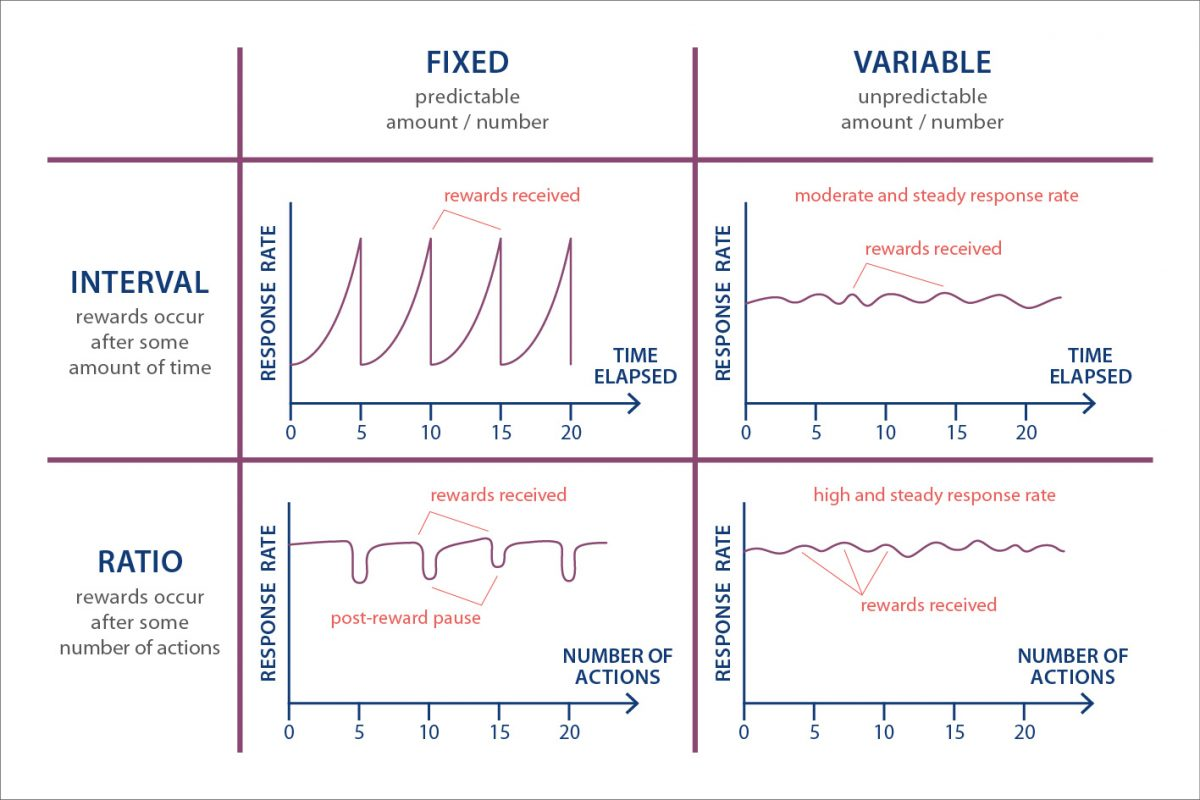
\includegraphics[width=14cm, height=8cm]{Graph.jpg}


\cite{hodent_2021}

\section{Gaming Disorder}
Addiction refers to pathological behavior that has a precise definition. There are addictions tied to the use of a substance, such as alcohol, opioids, or tobacco. In these addictions, the substance generally creates a physical dependence. For example, heroin binds to opioid receptors in the brain, creating a surge of pleasurable sensation. It is extremely addictive as it is disturbing the balance of hormonal and neuronal systems, and its impact cannot easily be reversed, creating a profound tolerance and physical dependence. Other substances don’t create such a dramatic physical dependence, or can create a dependence that is mainly psychological, which of course does not mean that their effects are less concerning.\cite{freeman2008internet}
Symptoms to diagnose an Internet gaming disorder are the following:
\begin{itemize}
    \item Preoccupation with gaming;
    \item Withdrawal symptoms when gaming is taken away or not possible (sadness, anxiety, irritability);
    \item Tolerance: need to spend more time gaming to satisfy the urge;
    \item Inability to reduce playing, unsuccessful attempts to quit gaming;
    \item Giving up other activities, loss of interest in previously enjoyed activities due to gaming;
    \item Continuing to game despite problems;
    \item Deceiving family members or others about the amount of time spent on gaming;
    \item The use of gaming to relieve negative moods, such as guilt or hopelessness;
    \item Risk, having jeopardized or lost a job or relationship due to gaming.
\end{itemize}

\section{Resolution}
Now that the problem has been identified, two questions remain: Should anything be done? and if so, What can be done to remedy this?
\subsection{Education}
An important aspect is the education to address the similar risk factors inherent in
gambling and gaming. Although the leisure and positive aspects of gambling are highlighted, marketed, and understood, the downside must also be emphasized, especially regarding gambling disguised as video or
social games.\cite{spekman2013gaming}
\subsection{Age Restriction}
Social gaming operators must be more socially responsible in how they market their
games and how they encourage in-game purchasing. Stricter age
verification measures should be in place for social games, especially where such
games allow young people to play games with gambling-related content (often with
exaggerated payout rates), even if real money is not used.
\subsection{Parental Advisory}
Parents also need to assume responsibility when allowing their children to play
social games or download gaming apps. Parents need to work with their children to prevent them from buying
in-game items for real money, including overseeing all apps they download, not
providing online store passwords, deleting stored credit and debit card information
from online accounts, and discussing buying in-game extras with their children. From a public health perspective, carefully monitoring the
behaviour of youth is highly recommended.
\subsection{Ethical Development}
And finally, the most important of all, us as ICT professionals needs to conserve our ethics and make sure that anything we program is for the benefit of society as a whole.
At the root of it all, we are the ones at the heart of development, and we possess the power to build software ethically. To quote IEEE: "The short version of the code summarizes aspirations at a high level of the abstraction; the clauses that are included in the full version give examples and details of how these aspirations change the way we act as software engineering professionals. Without the aspirations, the details can become legalistic and tedious; without the details, the aspirations can become high sounding but empty; together, the aspirations and the details form a cohesive code." \cite{ieee}


\section{Conclusion}
Through the research conducted in the numerous studies cited, it is evident that there may be a closer relation between gambling and features implemented in games, and in some cases the internet as a whole, than initially expected. There is also a lack of research on the psychological impact of these attention-grabbing tactics on children, and may promote the prevalence of addictive behavior in the youth if not regulated. 

\tableofcontents

\bibliographystyle{alpha}
\bibliography{sample}

\end{document}